%-----------------------------------LICENSE------------------------------------%
%   This file is part of tikz_figures.                                         %
%                                                                              %
%   tikz_figures is free software: you can redistribute it and/or              %
%   modify it it under the terms of the GNU General Public License as          %
%   published by the Free Software Foundation, either version 3 of the         %
%   License, or (at your option) any later version.                            %
%                                                                              %
%   tikz_figures is distributed in the hope that it will be useful,            %
%   but WITHOUT ANY WARRANTY; without even the implied warranty of             %
%   MERCHANTABILITY or FITNESS FOR A PARTICULAR PURPOSE.  See the              %
%   GNU General Public License for more details.                               %
%                                                                              %
%   You should have received a copy of the GNU General Public License along    %
%   with tikz_figures.  If not, see <https://www.gnu.org/licenses/>.           %
%------------------------------------------------------------------------------%

% Use the standalone class for displaying the tikz image on a small PDF.
\documentclass[crop, tikz]{standalone}

% Import the tikz package to use for the drawing.
\usepackage{tikz}

% Begin the document.
\begin{document}

    % Begin the drawing.
    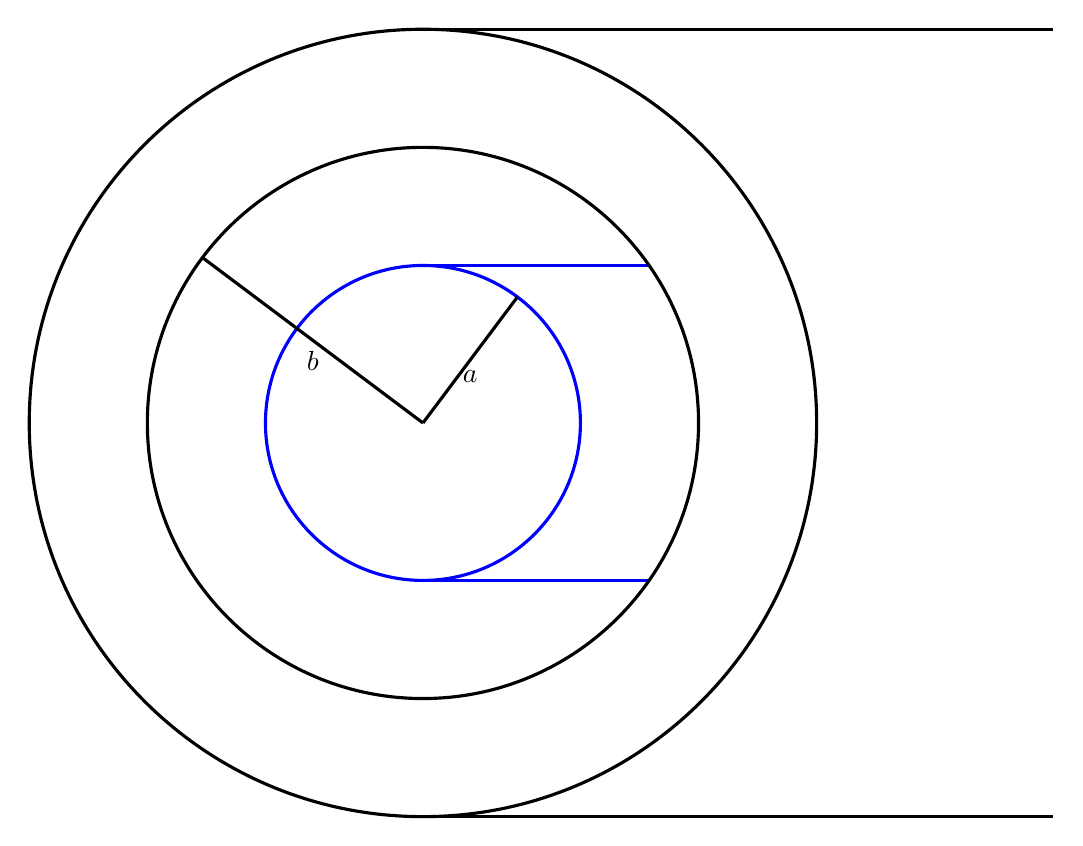
\begin{tikzpicture}[line width = 0.4mm]

        % Circle and two clipped lines for the inner solid cylinder.
        \draw[blue] (0.0, 0.0) circle (2.0);
        \draw[blue] (0.0, 2.0) to (2.88, 2.0);
        \draw[blue] (0.0, -2.0) to (2.88, -2.0);

        % Two circles for the outer hollow cylinder.
        \draw (0.0, 0.0) circle (3.5);
        \draw (0.0, 0.0) circle (5);

        % Radial lines for the two cylinders.
        \draw (0.0, 0.0) to node [below] {$a$} (1.2, 1.6);
        \draw (0.0, 0.0) to node [below] {$b$} (-2.8, 2.1);

        % Vertical lines for the outer cylinder.
        \draw (0.0, -5.0) to (8.0, -5.0);
        \draw (0.0, 5.0) to (8.0, 5.0);
    \end{tikzpicture}
\end{document}
